\newpage
\section{Programm Umsetzung}
Das Programm wurde wie angegeben in 4 Threads eingeteilt.
\begin{itemize}
    \item Main-Thread
    \begin{itemize}
        \item Initialisierung der anderen Threads
        \item UART und Crypto Device Initialisierung 
        \item Validate Hardware Compatibility 
        \item alle 5 Sekunden ein Lebenszeichen von sich geben. 
    \end{itemize} 
    \item UART-IN-Thread
    \item UART-OUT-Thread
    \item PROCESS-Thread
\end{itemize}
\subsection{Blockschaltbild}
\begin{figure}[!ht]
    \centering
    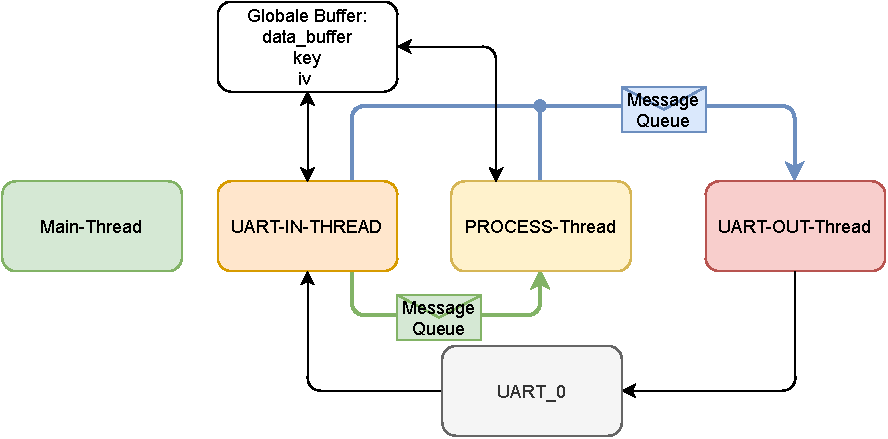
\includegraphics[width=\linewidth]{Blockschaltbild.pdf}
    \caption{Blockschaltbild}
    \label{fig:Blockschaltbild}
\end{figure}

\subsection{Projekt Konfiguration}
\subsection{Initialisierung}
\subsection{UART-In-Thread}
\subsection{UART-Out-Thread}
\subsection{Processing Thread}
\subsubsection{Entschlüsselung}

\subsection{Test-Ausführung}